%! Author = mariuszindel
%! Date = 02.11.20

\section{Entity Framework Core}


\subsection{Überblick}
\begin{itemize}
    \item Entity Framework Core / EF Core ist ein O/R Mapping Framework
    \begin{itemize}
        \item Verbindet Objekt-Orientiertes (Domain Model)
        \item mit Relationalem (Relational Model)
    \end{itemize}
    \item Diverse Basis-Funktionalitäten
    \begin{itemize}
        \item Mapping von Entitäten
        \item CRUD Operationen (Create, Read, Update, Delete
        \item Key-Generierung
        \item Caching
        \item Change Tracking
        \item Optimistic Concurrency
        \item Transactions
        \item Command Line Interface
    \end{itemize}
\end{itemize}


\subsection{OR-Mapping}

\subsubsection{Providers}
\begin{center}
    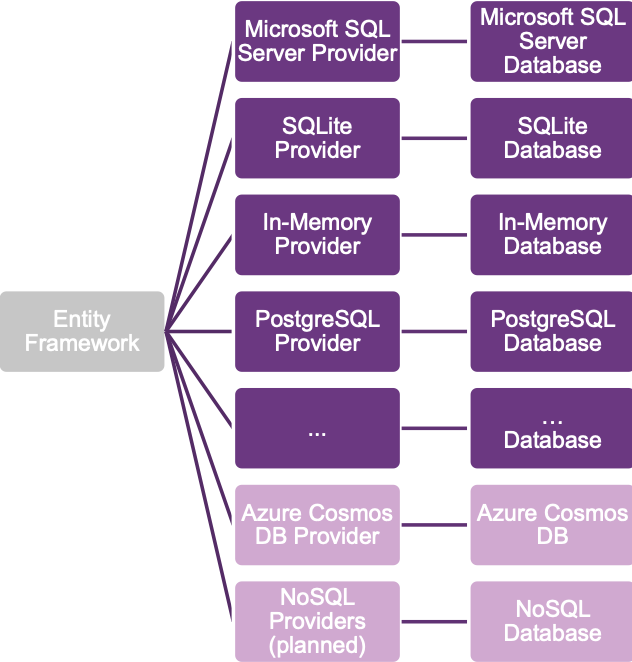
\includegraphics[scale=.4]{graphic/efc/providers.png}
\end{center}
\vspace{-8pt}

\subsubsection{Überblick}
\begin{itemize}
    \item Entity Type
    \begin{itemize}
        \item Domain Modell / Konzeptionelles Modell / etc.
        \item Normale .NET Klassen
    \end{itemize}
    \item Mapping - Drei verschiedene Ansätze:
    \begin{itemize}
        \item By Convention
        \item By Attributes
        \item By Fluent API
    \end{itemize}
    \item Storage Entity
    \begin{itemize}
        \item Relationales Modell / Graph / Collection / etc.
        \item Abhängig von gewähltem Provider
    \end{itemize}
\end{itemize}
\vspace{-8pt}
\begin{center}
    \includegraphics[scale=.3]{graphic/efc/überblick.png}
\end{center}
\vspace{-8pt}

\subsubsection{Entrity Type}
\begin{itemize}
    \item Ausprägung
    \begin{itemize}
        \item Klasse
    \end{itemize}
    \item Inhalte
    \begin{itemize}
        \item Properties (Name)
        \item Entry Keys (Primary Key)
        \item Alternative Keys
        \item Relationships
        \item Foreign Keys
    \end{itemize}
\end{itemize}

\subsubsection{Storage Entity}
\begin{itemize}
    \item Ausprägung
    \begin{itemize}
        \item Table
        \item View
        \item Stored Procedures
    \end{itemize}
    \item Inhalte
    \begin{itemize}
        \item Columns
        \item Primary Keys
        \item Unique Key Constraints
        \item Foreign Keys
    \end{itemize}
\end{itemize}

\subsubsection{Mapping}
\begin{itemize}
    \item Zuordnung von
    \begin{itemize}
        \item Entity Type zu Storage Entity
        \item Property zu Column
        \item Entity Key zu Primary Key
        \item Foreign Key zu Relationship
    \end{itemize}
    \item Erweiterte Szenarien
    \begin{itemize}
        \item Vererbung / Inheritance
        \item Table Split / Table Merge
        \item Complex Types
    \end{itemize}
    \item Ausprägungen
    \begin{itemize}
        \item By Convention
        \item By Attributes
        \item By Fluent API
    \end{itemize}
\end{itemize}

\subsubsection{Mappingarten (Entity-Level)}
\begin{center}
    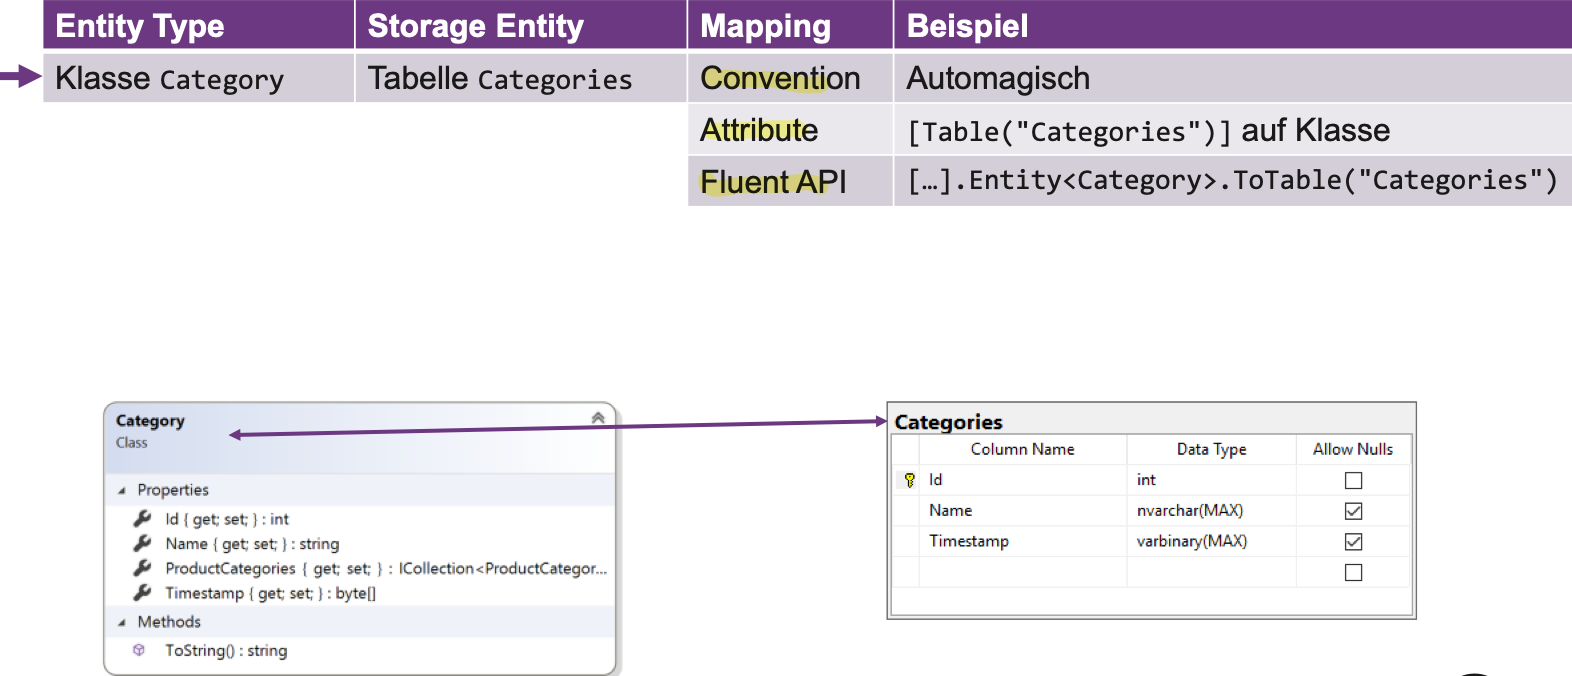
\includegraphics[scale=.32]{graphic/efc/Entity-Level.png}
\end{center}
\vspace{-8pt}

\subsubsection{Mappingarten (Attribut-Level)}
\begin{center}
    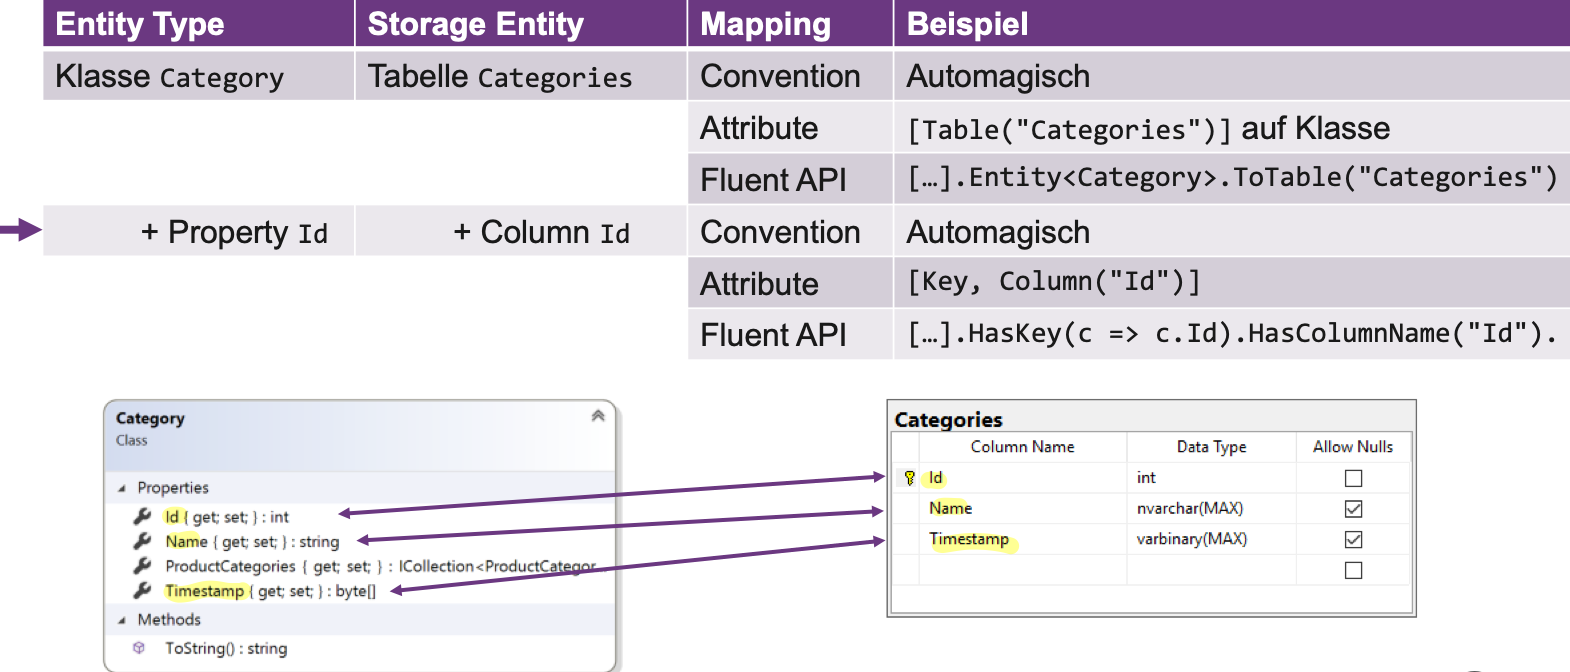
\includegraphics[scale=.32]{graphic/efc/Attribut-Level.png}
\end{center}
\vspace{-8pt}

\subsection{Ansätze}
\begin{center}
    \includegraphics[scale=.3]{graphic/efc/ansätze.png}
\end{center}
\vspace{-8pt}


\subsection{OR-Mapping Modell}
\subsubsection{Überblick}
\begin{itemize}
    \item Mapping by Convention
    \begin{itemize}
        \item Automatisches Mapping ohne explizite Konfiguration
    \end{itemize}
    \item Mapping by Fluent API
    \begin{itemize}
        \item Extension-Method-Syntax
        \item Überschriebene Methode von «OnModelCreating» im DbContext
    \end{itemize}
    \item Mapping by Data Annotations
    \begin{itemize}
        \item Deklaratives Mapping
        \item Attribute direkt auf Model-Klassen
        \item Namespace
    \end{itemize}
\end{itemize}

\subsubsection{Include / Exclude von Entities}
\begin{center}
    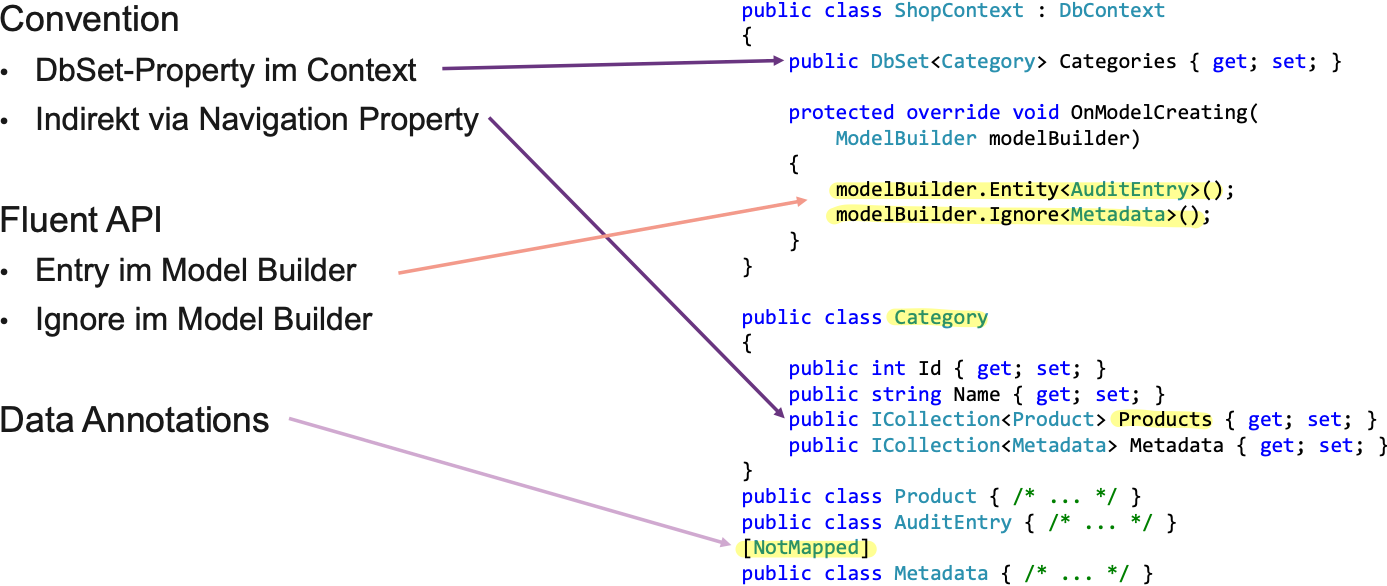
\includegraphics[scale=.35]{graphic/efc/Include Exclude von Entities.png}
\end{center}
\vspace{-8pt}

\subsubsection{Include / Exclude von Properties}
\begin{center}
    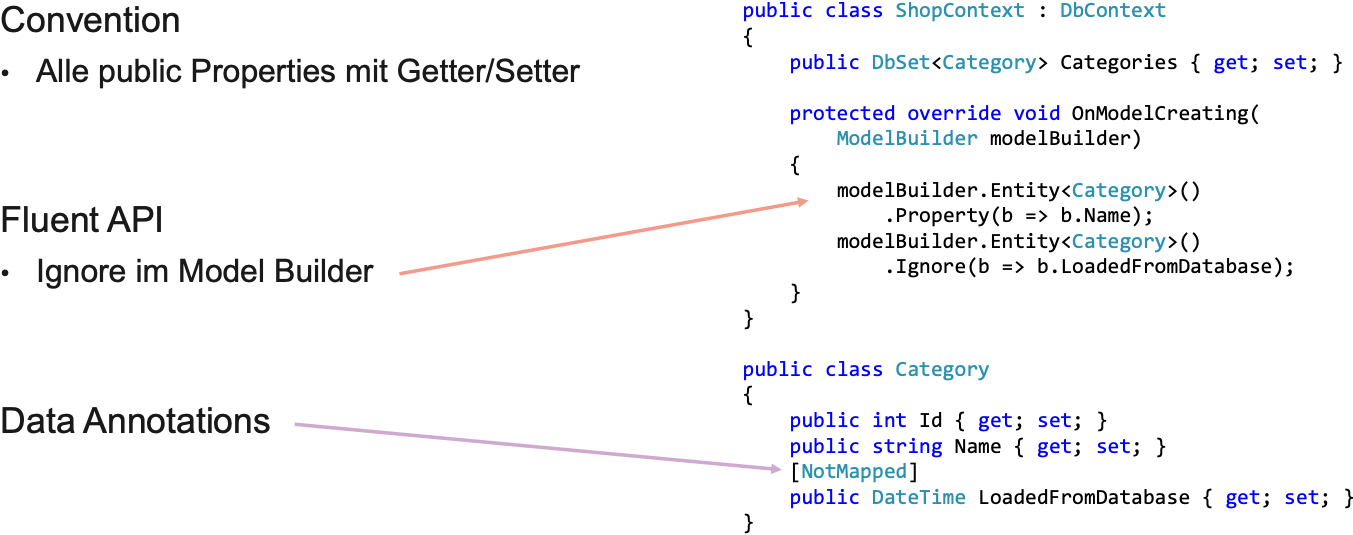
\includegraphics[scale=.35]{graphic/efc/Include Exclude von Properties.png}
\end{center}
\vspace{-8pt}

\subsubsection{Keys}
\begin{center}
    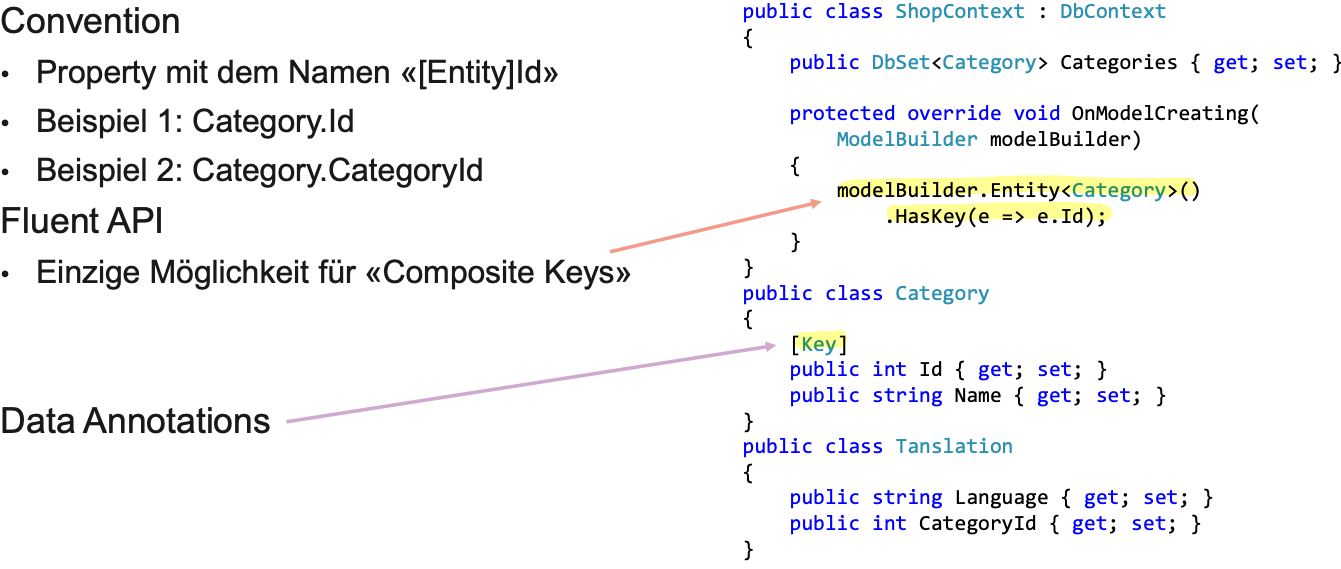
\includegraphics[scale=.37]{graphic/efc/Keys.png}
\end{center}
\vspace{-8pt}

\subsubsection{Required / Optional}
\begin{center}
    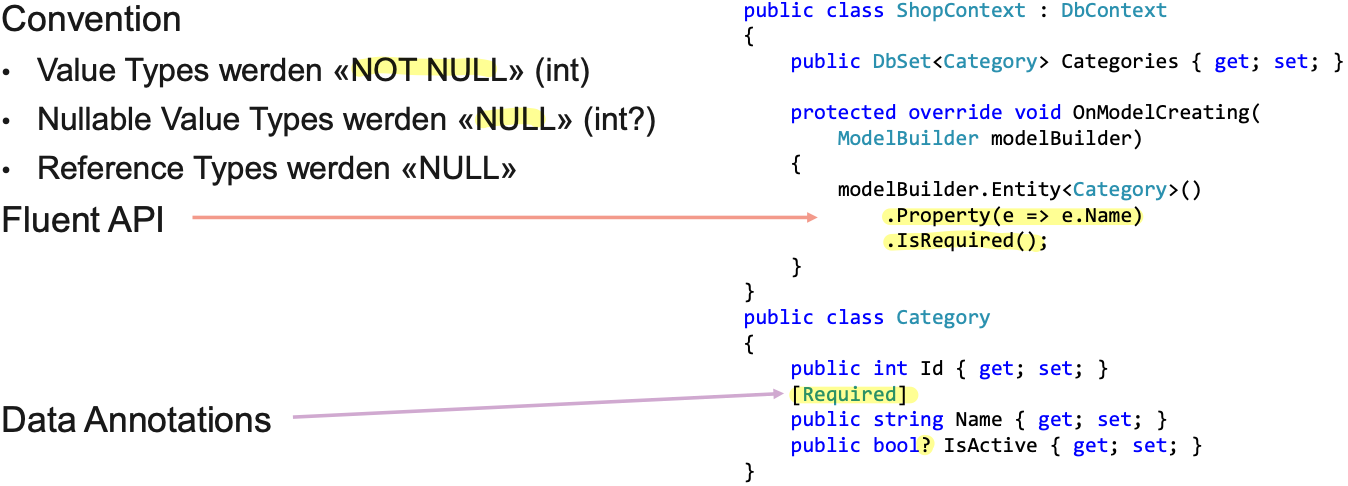
\includegraphics[scale=.37]{graphic/efc/Required Optional.png}
\end{center}
\vspace{-8pt}

\subsubsection{Maximum Length}
\begin{center}
    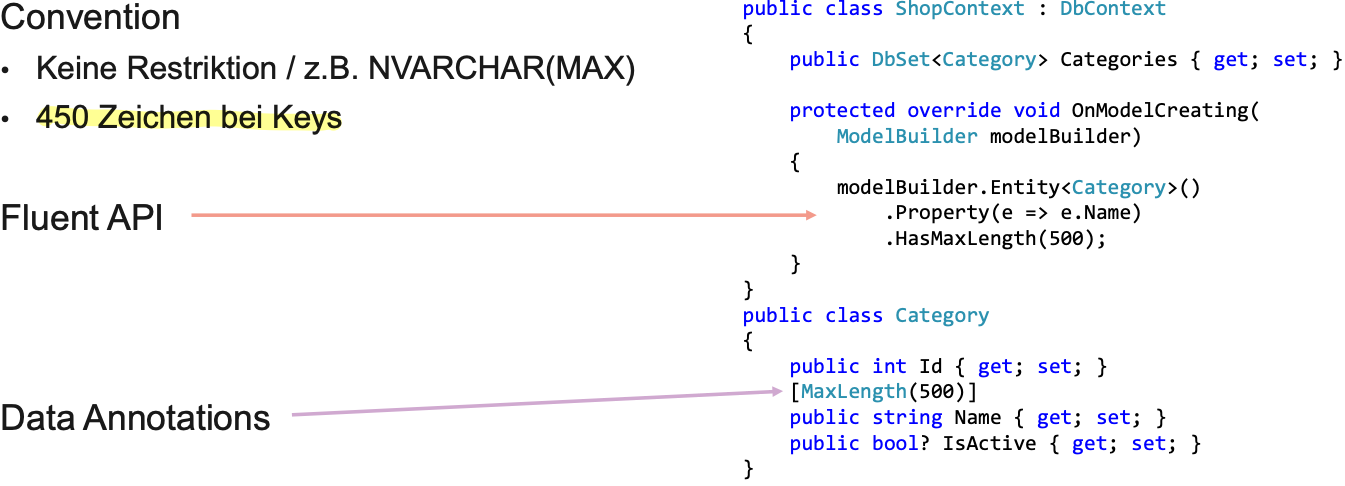
\includegraphics[scale=.37]{graphic/efc/Maximum Lengt.png}
\end{center}
\vspace{-8pt}

\subsubsection{Indexes}
\begin{center}
    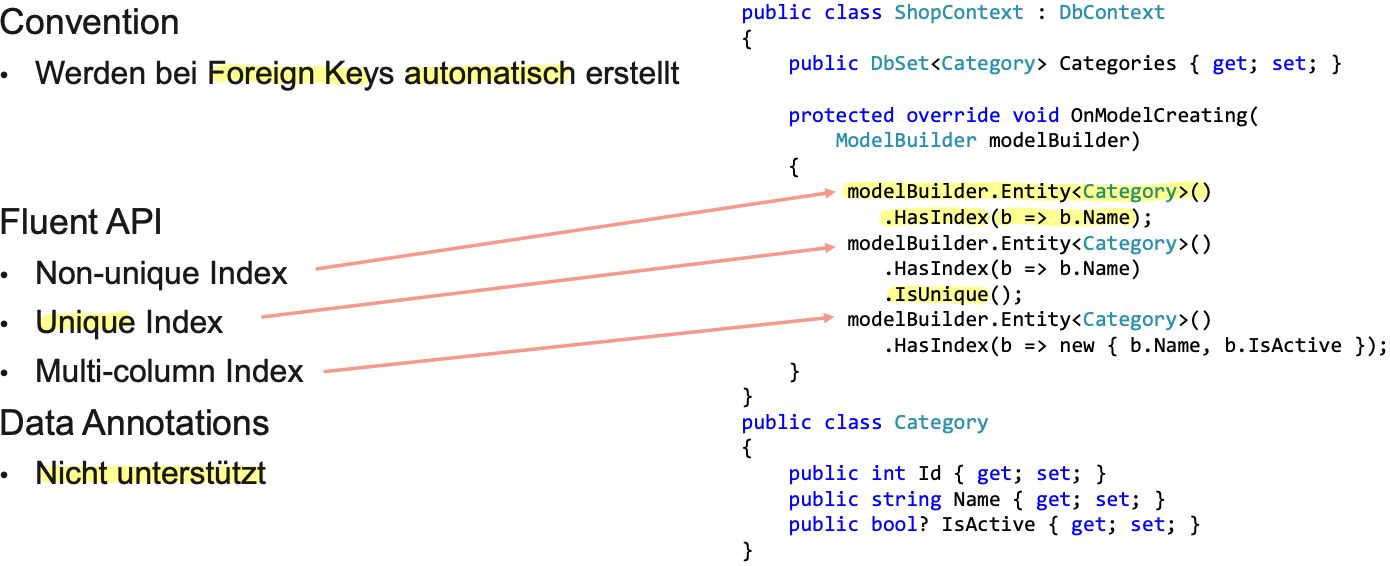
\includegraphics[scale=.36]{graphic/efc/Indexes.png}
\end{center}
\vspace{-8pt}

\subsubsection{Entity Type Configuration}
\begin{center}
    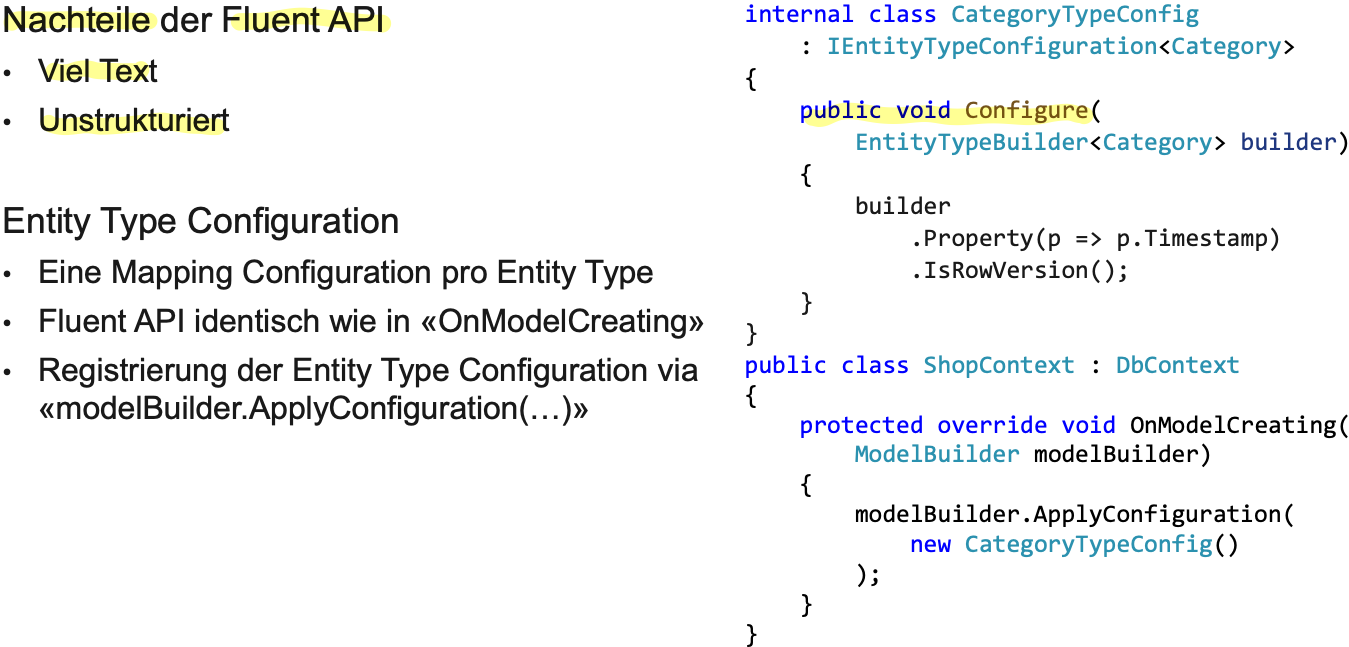
\includegraphics[scale=.37]{graphic/efc/Entity Type Configuration.png}
\end{center}
\vspace{-8pt}


\subsection{OR-Mapping: Relationale Datenbank (SQL Server)}

\subsubsection{Tabellen}
\begin{center}
    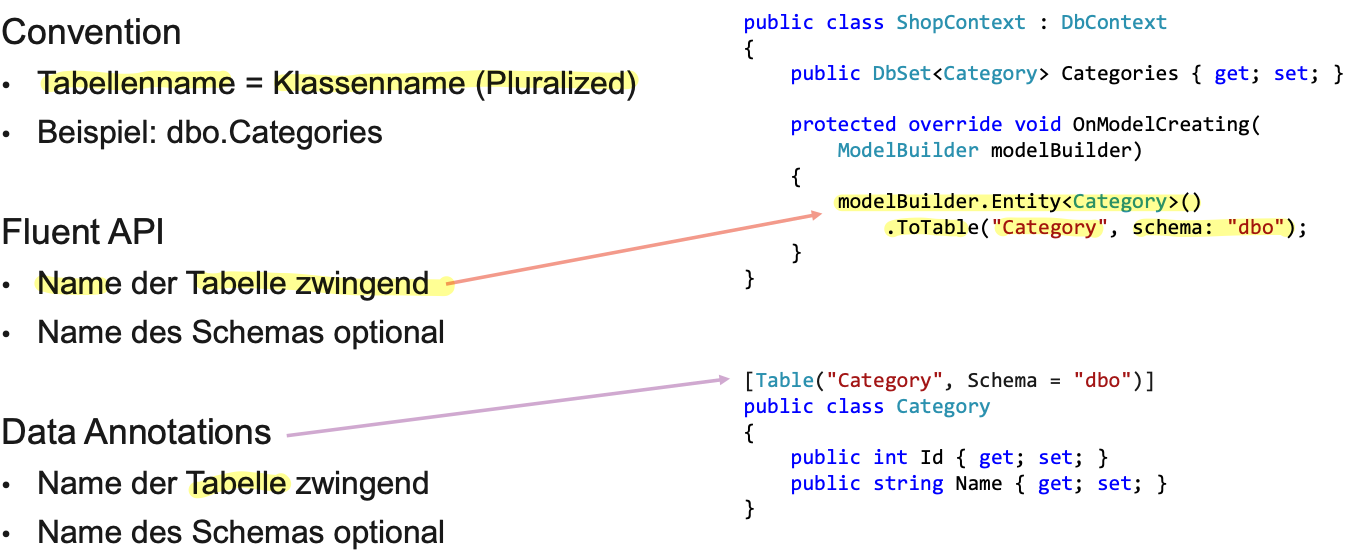
\includegraphics[scale=.37]{graphic/efc/tabellen.png}
\end{center}
\vspace{-8pt}

\subsubsection{Spalten}
\begin{center}
    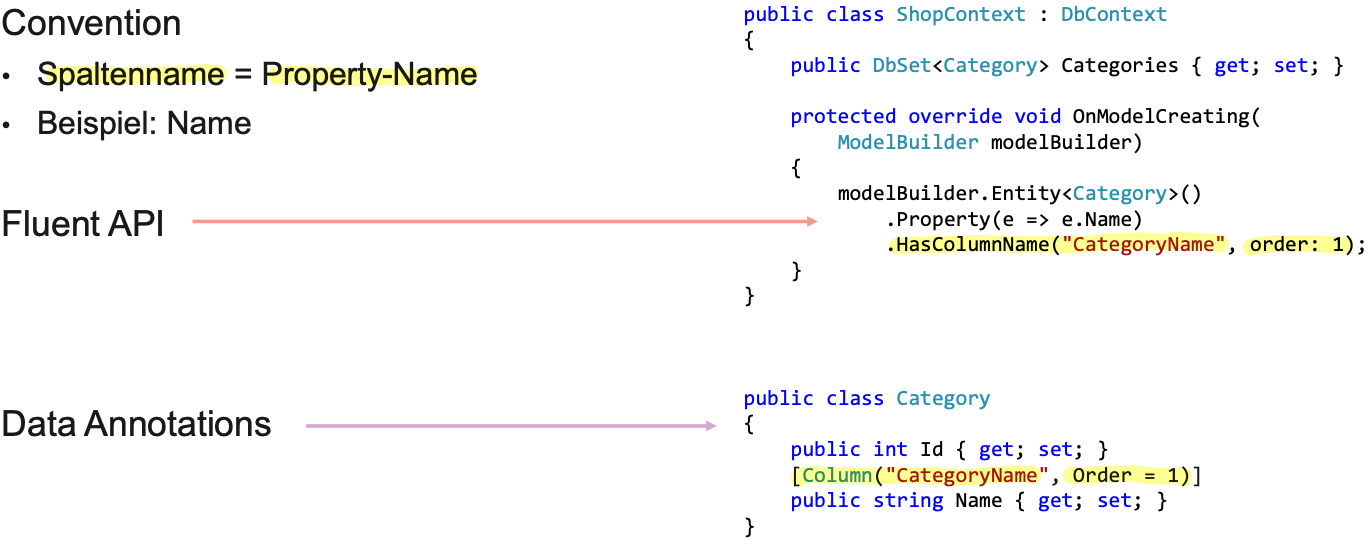
\includegraphics[scale=.37]{graphic/efc/Spalten.png}
\end{center}
\vspace{-8pt}

\subsubsection{Datentypen / Default Values}
\begin{center}
    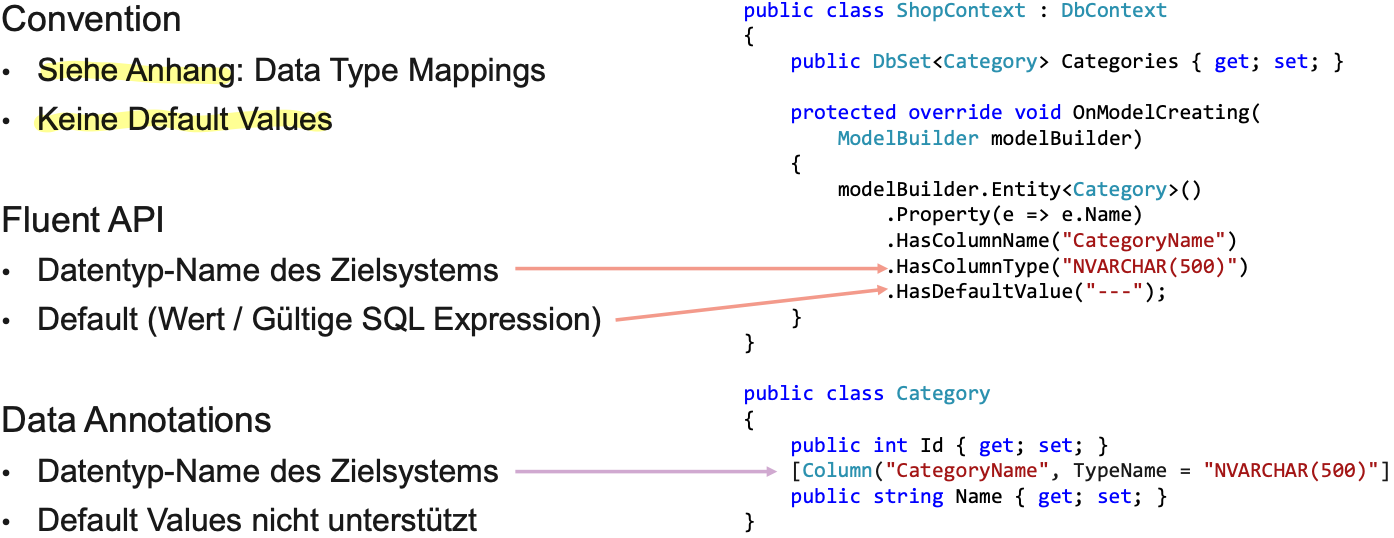
\includegraphics[scale=.37]{graphic/efc/Datentypen Default Values.png}
\end{center}
\vspace{-8pt}

\subsubsection{Relationship – one-to-many / Fully Defined}
\begin{center}
    \includegraphics[scale=.37]{graphic/efc/Relationship – one-to-many Fully Defined.png}
\end{center}
\vspace{-8pt}

\subsubsection{Relationship – one-to-many / No Foreign Key Property}
\begin{center}
    \includegraphics[scale=.37]{graphic/efc/Relationship – one-to-many No Foreign Key Property.png}
\end{center}
\vspace{-8pt}

\subsubsection{Relationship – one-to-many / Single Navigation Property}
\begin{center}
    \includegraphics[scale=.37]{graphic/efc/Relationship – one-to-many Single Navigation Property.png}
\end{center}
\vspace{-8pt}

\subsubsection{Relationship – one-to-many / Foreign Key}
\begin{center}
    \includegraphics[scale=.36]{graphic/efc/Relationship – one-to-many Foreign Key.png}
\end{center}
\vspace{-8pt}

\subsubsection{Relationship – one-to-one / many-to-many}
\begin{center}
    \includegraphics[scale=.3]{graphic/efc/Relationship – one-to-one many-to-many.png}
\end{center}
\vspace{-8pt}

\subsubsection{Relationship – Diverses}
\begin{center}
    \includegraphics[scale=.31]{graphic/efc/Relationship – Diverses.png}
\end{center}
\vspace{-8pt}

\subsubsection{Diverses}
\begin{center}
    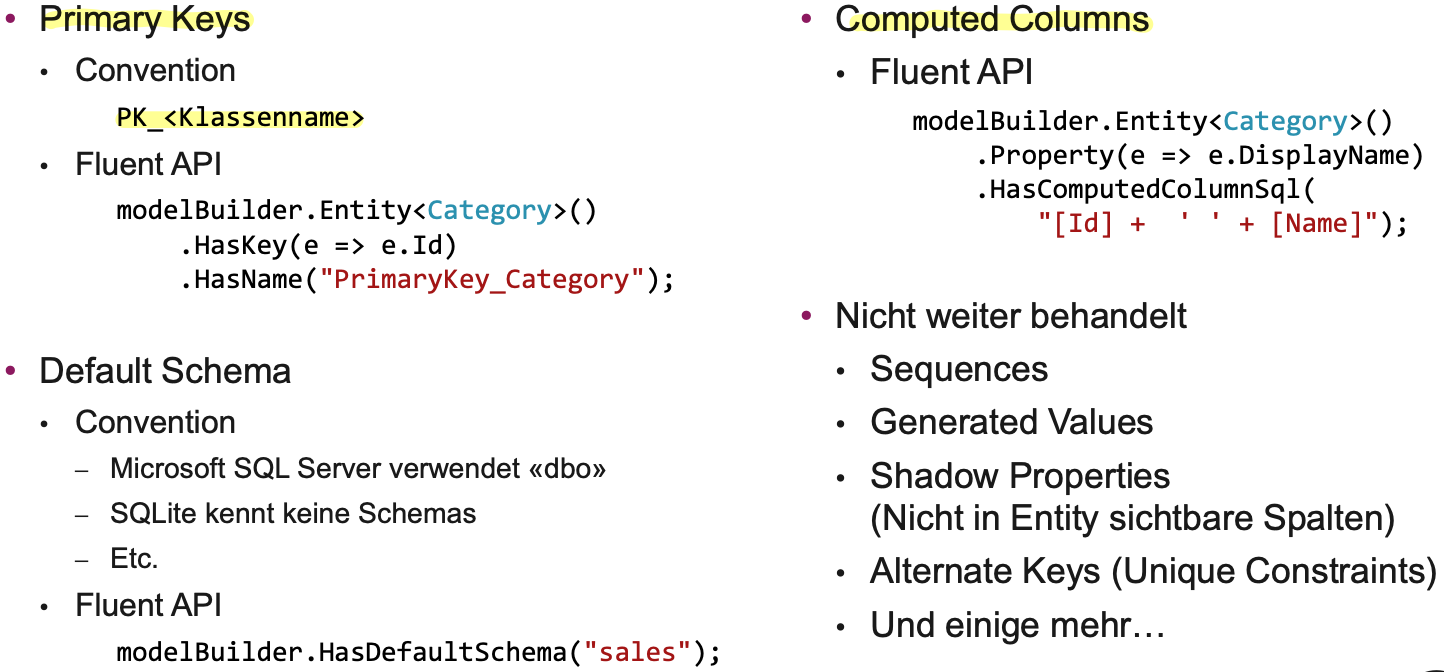
\includegraphics[scale=.33]{graphic/efc/Diverses.png}
\end{center}
\vspace{-8pt}


\subsection{Database Context}

\subsubsection{Überblick}
\begin{itemize}
    \item Wichtigster Teil des Entity Framework
    \item Kombination zweier Patterns
    \begin{itemize}
        \item Repository + Unit of Work
    \end{itemize}
    \item Funktionen:
    \begin{itemize}
        \item Design-Time
        \begin{itemize}
            \item Model definieren (OR-Mapping)
            \item Konfiguration
            \item Database Migrations
        \end{itemize}
        \item Run-Time
        \begin{itemize}
            \item Connections verwalten (Connection Pool)
            \item CRUD Operationen ausführen
            \item Change Tracking
            \item Caching
            \item Transaction Management
        \end{itemize}
    \end{itemize}
\end{itemize}

\subsubsection{DbContext Lifecycle}
DbContext-Instanzen sollten nicht
\begin{itemize}
    \item zu lange leben
    \begin{itemize}
        \item Limitierte Anzahl Connections im Client Connection Pool
        \item Change-Tracking wird über die Zeit ineffizient
    \end{itemize}
    \item geshared werden
    \begin{itemize}
        \item Ist nicht thread-safe
        \item Exception kann Instanz unbrauchbar machen
    \end{itemize}
\end{itemize}

Empfehlungen:
\begin{itemize}
    \item In einem «using»-Statement verwenden
    \item Web Applikationen: Instanz pro Request
    \item GUI: Instanz pro Formular
    \item Generell: Instanz pro «Unit of Work»
\end{itemize}
\begin{lstlisting}
// So verwenden:
using (ShopContext context = new ShopContext()) { Query... }
\end{lstlisting}


\subsection{Query Execution with JOIN}
\begin{center}
    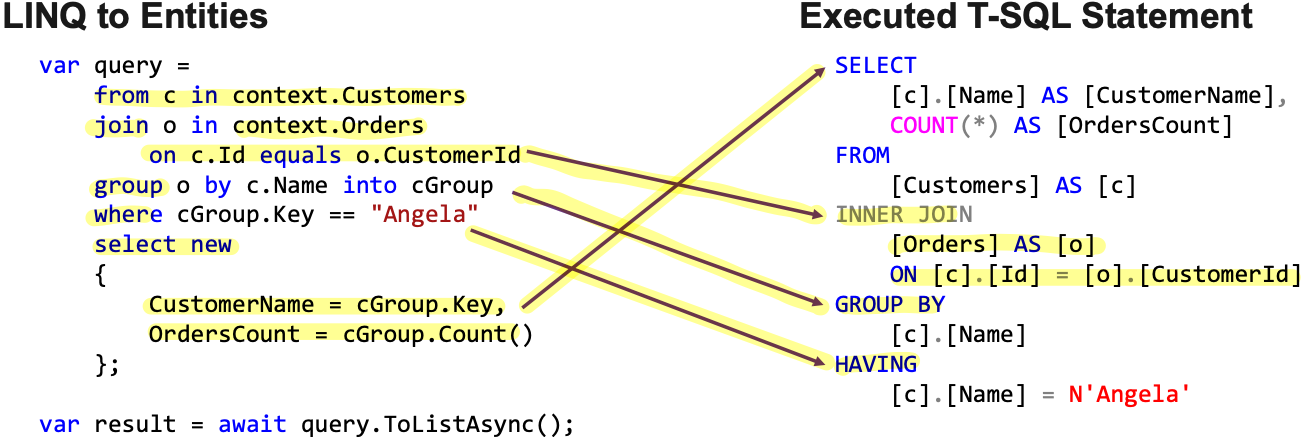
\includegraphics[scale=.35]{graphic/efc/join.png}
\end{center}
\vspace{-8pt}

\subsection{Database Context: CUD Operatoren}
\subsubsection{Insert}
\begin{lstlisting}
using (ShopContext context = new ShopContext()) {
    Category cat = new Category
        { Name = "Notebooks" };

    // Add to Context (3 alternatives)
    context.Add(cat);
    context.Categories.Add(cat);
    context.Entry(cat).State = EntityState.Added;

    // Save - SQL is executed here
    await context.SaveChangesAsync();

    // Check Primary Key
    int id = cat.Id; // Category.Id is populated
}
\end{lstlisting}

\subsubsection{Update}
\begin{lstlisting}
using (ShopContext context = new ShopContext()) {
    Category cat = await context
        .Categories
        .FirstAsync(); £$\rightarrow$ .Single(p=>p.Name == "Hans");£

    // Change
    cat.Name = "Changed";

    // Save - SQL is executed here
    await context.SaveChangesAsync(); £$\rightarrow$ Oder auch ohne Async£
}
\end{lstlisting}

\subsubsection{Delete}
\begin{lstlisting}
using (ShopContext context = new ShopContext()) {
    Category cat = await context
        .Categories
        .FirstAsync(c => c.Name == "Notebooks");

    // Remove (3 alternatives)
    context.Remove(cat);
    context.Categories.Remove(cat);
    context.Entry(cat).State = EntityState.Deleted;

    // Save - SQL is executed here
    await context.SaveChangesAsync();
}
\end{lstlisting}


\subsection{Database Context: Change Relationship II}
\begin{itemize}
    \item Via Navigation Property
    \item Via Foreign Key
\end{itemize}

\subsection{Database Context: Change Tracking}
\subsubsection{Überblick}
Change Tracker:
\begin{itemize}
    \item Registriert alle Ändungen an «getrackten» Entities
    \item Aktualisiert den Entity State
    \item • Agiert komplett «offline»
\end{itemize}
State Handling:
\begin{itemize}
    \item DbContext hat Methoden für das Hinzufügen und das Setzen des States im Change Tracker
    \begin{itemize}
        \item Add()
        \item Remove()
        \item Update()
        \item Unchanged()
    \end{itemize}
    \item Immer mind. 3 Varianten mit gleichem Effekt
    \begin{itemize}
        \item .Add / .Remove / etc. berücksichtigen ganzen Objekt-Graphen 
        \item .Entry(…).State nur die jeweilige Entity
    \end{itemize}
\end{itemize}
\vspace{-8pt}
\begin{center}
    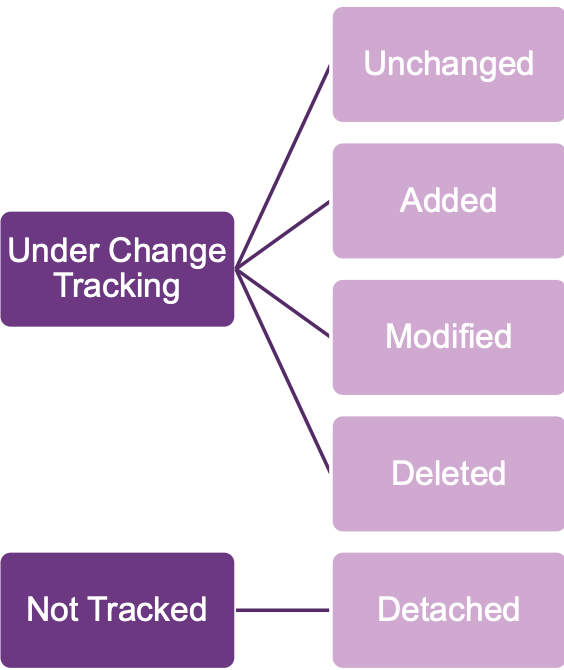
\includegraphics[scale=.3]{graphic/efc/change tracker.png}
\end{center}
\vspace{-8pt}

\subsubsection{State Entries}
\begin{itemize}
    \item Via DbContext.Entry<T>(object)...
    \item Beinhaltet Informationen über
    \begin{itemize}
        \item Status des Objekts
        \item Für alle Properties
        \begin{itemize}
            \item
        \end{itemize}
        \item Entity-specific loading functions
        \item Reload object values from database
        \item Load referenced entities (see explicit lazy loading)
    \end{itemize}
\end{itemize}
\vspace{-8pt}
\begin{center}
    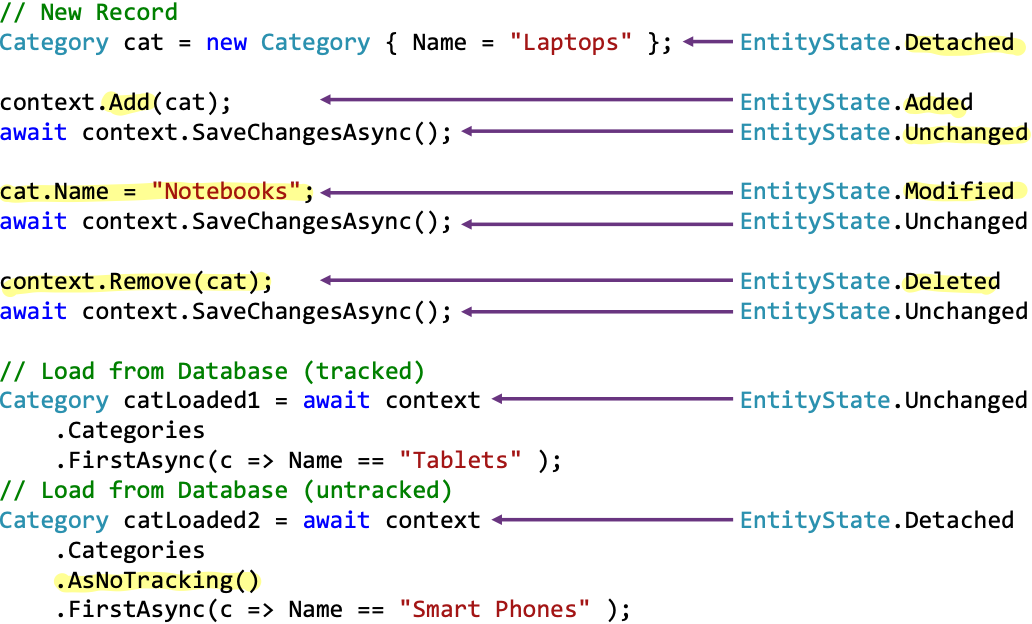
\includegraphics[scale=.44]{graphic/efc/state entries.png}
\end{center}
\vspace{-8pt}

%\columnbreak

\subsection{Database Context: Ladestrategien}

\subsubsection{Überblick}
Was wird beim Laden eines «Order» Objekts geladen?
\begin{lstlisting}
Order order = await context
    .Orders
    .FirstAsync();

var customer = order
    .Customer; // customer is "null"

var items = order
    .Items; // items is "null"
\end{lstlisting}

\subsubsection{Eager Loading (Default)}
\begin{itemize}
    \item Assoziationen werden per se nicht geladen
    \item Include()-Statement für einzelne Assoziationen
    \item Passiert in der gleichen Abfrage per JOIN
\end{itemize}
\vspace{-8pt}
\begin{center}
    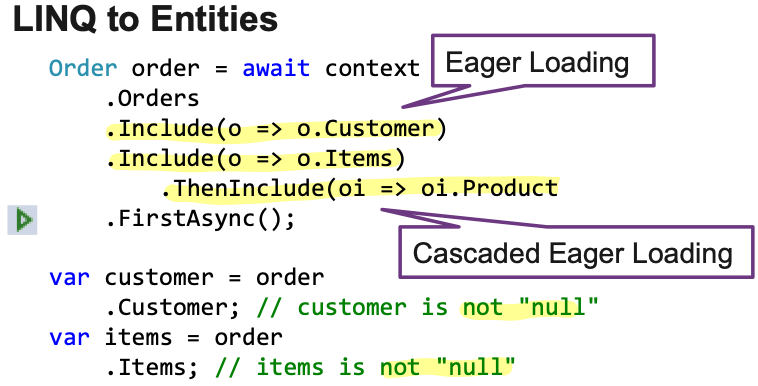
\includegraphics[scale=.4]{graphic/efc/eager loading.png}
\end{center}
\vspace{-8pt}

\subsubsection{Explicit Loading}
\begin{itemize}
    \item Assoziationen werden per se nicht geladen
    \item Assoziationen werden explizit nachgeladen
    \item Collections werden komplett geladen
    \item Passiert in separater Abfrage
\end{itemize}
\vspace{-8pt}
\begin{center}
    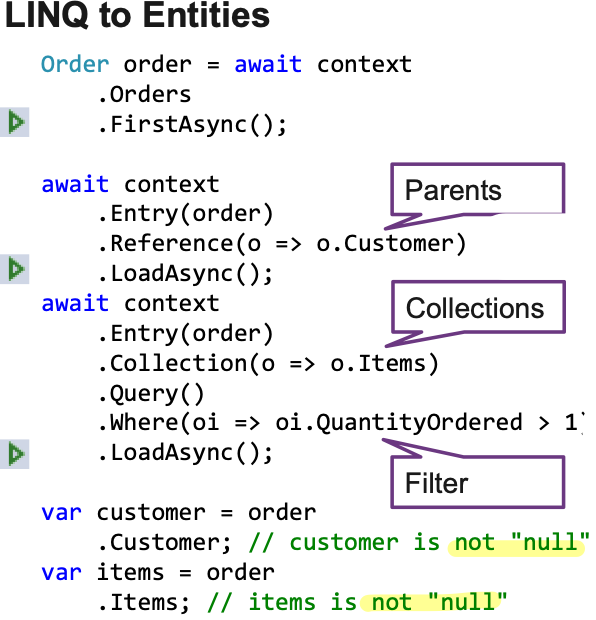
\includegraphics[scale=.4]{graphic/efc/explicit loading.png}
\end{center}
\vspace{-8pt}

\subsubsection{Lazy Loading}
\begin{itemize}
    \item Assoziationen werden per se nicht geladen
    \item Assoziationen werden bei Zugriff auf Property automatisch nachgeladen
    \item Collections werden komplett geladen / Filtern aber möglich
    \item Passiert in separater Abfrage
\end{itemize}
Problem:
\begin{itemize}
    \item Model-Klassen meist mit Auto-Properties
    \item Wie kann bei Zugriff auf ein Property zusätzliche (Lade-)Logik ausgeführt werden
\end{itemize}
2 Lösungsvarianten:

\subsubsection{Lazy Loading – Manuell}
Auf Auto-Properties verzichten und Logik manuell implementieren
\vspace{-8pt}
\begin{center}
    \includegraphics[scale=.21]{graphic/efc/Lazy Loading – Manuell.png}
\end{center}
\vspace{-8pt}

\subsubsection{Lazy Loading – Proxy}
\begin{itemize}
    \item Dynamic Binding
    \item Navigation Properties mit «virtual» Keyword
    \item EF Core generiert abgeleitete Proxy-Klassen $\rightarrow$ Zur Laufzeit generiert mit «Castle»
    \item Diese enthalten ca. die Logik von Variante 1
\end{itemize}
\vspace{-8pt}
\begin{center}
    \includegraphics[scale=.21]{graphic/efc/Lazy Loading – Proxy.png}
\end{center}
\vspace{-8pt}

\subsection{Optimistic Concurrency}
\subsubsection{Überblick}
\begin{itemize}
    \item Annahme:
    \begin{itemize}
        \item Zwischen Laden und Speichern eines Records wird nicht verändert $\rightarrow$ Beim Speichern prüfen, ob geändert
    \end{itemize}
    \item Alternative: Pessimistic Concurrency
    \begin{itemize}
        \item Datensatz wird für die Dauer der Verarbeitung gesperrt
        \item Probleme
        \begin{itemize}
            \item Deadlocks
            \item Orphaned Locks
            \item Performance
        \end{itemize}
    \end{itemize}
\end{itemize}

\subsubsection{Erkennung von Konflikten: Timestamp}
\begin{itemize}
    \item Pro Record Timestamp / Row Version
    \item Timestamp ist Teil des Datenobjekts
    \item Datenbank-Timestamp = Objekt-Timestamp $\rightarrow$ Ja $\rightarrow$ speichern + timestamp erhöhen
\end{itemize}
\vspace{-8pt}
\begin{center}
    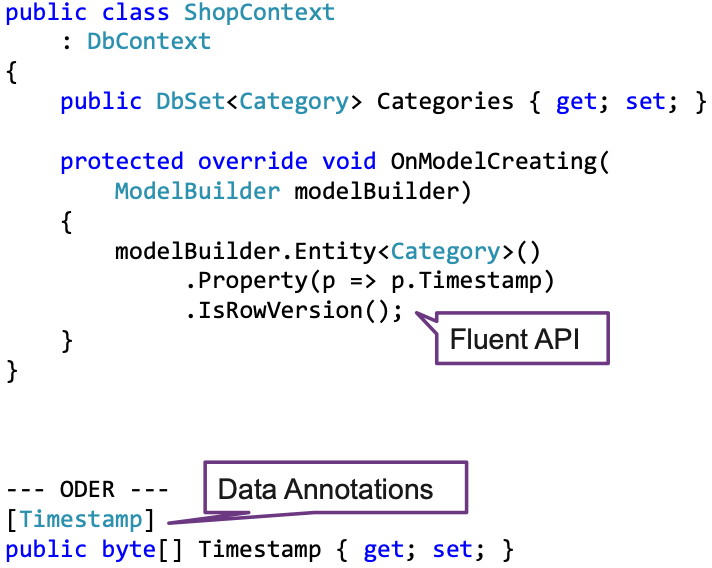
\includegraphics[scale=.38]{graphic/efc/timestamp.png}
\end{center}
\vspace{-8pt}

\subsubsection{Erkennung von Konflikten: Concurrency Tokens / Daten-Versionen}
\begin{itemize}
    \item Beim Ändern der Daten: Originalwerte wegkopieren
    \item Beim Speichern ebenfalls mitgeben
    \item Datenbankwerte = Originalwerte $\rightarrow$ Ja $\rightarrow$ speichern
\end{itemize}
\vspace{-8pt}
\begin{center}
    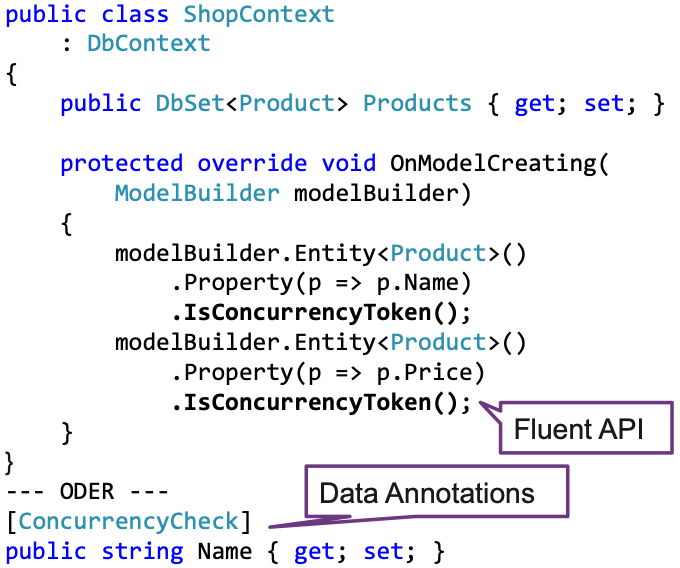
\includegraphics[scale=.4]{graphic/efc/Concurrency Tokens.png}
\end{center}
\vspace{-8pt}

\subsubsection{Optimistic Concurrency – Konfliktbehandlung}
DbUpdateConcurrencyException beinhaltet fehlerhafte «Entries»
\begin{itemize}
    \item Aktuelle Werte (vom zu speichernden Objekt)
    \item Original-Werte (ursprünglich geladene Werte)
    \item Datenbank-Werte (aktuell aus Datenbank)
\end{itemize}
Lösung:
\begin{itemize}
    \item Standardverfahren 1: Ignorieren
    \item Standardverfahren 2: Benutzer fragen
    \item Standardverfahren 3: Autokorrektur
\end{itemize}


\subsection{OR-Mapping Inheritance}
\subsubsection{Überblick}
\begin{itemize}
    \item Relationale Systeme kennen keine Vererbung
    \item Vorteil: Constraints können über Vererbung abgebildet werden
    \item Drei verschiedene Ansätze
\end{itemize}

\subsubsection{Table per Hierarchy}
\begin{itemize}
    \item Eine Tabelle pro Vererbungs-Hierarchie (EF Core Standard)
    \item Nur über DbContext definierbar
    \item Diskriminator zur unterscheidung notwendig (Default: Name der Klasse)
\end{itemize}

\subsubsection{Table per Type}
noch nicht implementiert!
\vspace{-8pt}
\begin{center}
    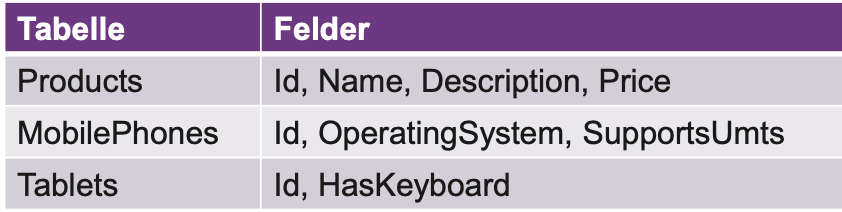
\includegraphics[scale=.32]{graphic/efc/Table per Type.png}
\end{center}
\vspace{-8pt}

\subsubsection{Table per Concrete Type}
noch nicht implementiert!
\vspace{-8pt}
\begin{center}
    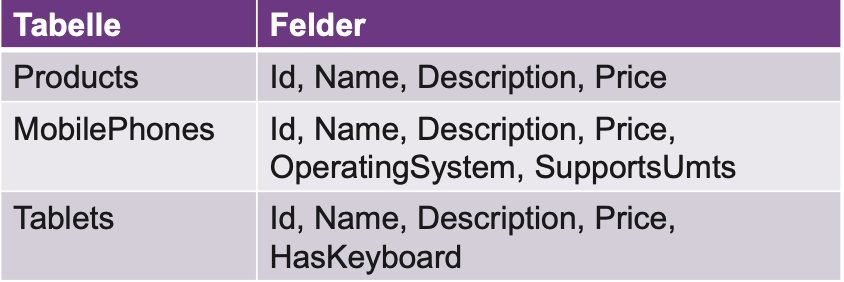
\includegraphics[scale=.32]{graphic/efc/Table per Concrete Type.png}
\end{center}
\vspace{-8pt}


\subsection{Database Migrations}
\subsubsection{Ansatz}
\begin{itemize}
    \item Während Entwicklung
    \begin{itemize}
        \item Modell anpassen
        \item Migration erstellen
        \begin{itemize}
            \item
        \end{itemize}
        \item Review der Migration
        \item Eventuelle Korrekturen anbringen
        \item Sourcecode Artefakt (Versionsverwaltung)
    \end{itemize}
    \item Deployment
    \begin{itemize}
        \item Änderungen gemäss Migration-Reihenfolge auf Datenbank deployen
        \item Rollback auf älteren Stand via Down-Migration möglich
    \end{itemize}
\end{itemize}

\newpage